\chapter{Test computazionali}
\label{cap:verifica-validazione}

\intro{In questo capitolo vengono descritte le istanze utilizzate per i test, la configurazione utilizzata per i parametri dell'algoritmo e i risultati ottenuti}

\section{Caratteristiche delle istanze}

Le classi di istanze utilizzate per i test computazionali dell'algoritmo sono caratterizzate da una combinazione di parametri che definiscono la complessità e la struttura del problema. Ogni classe rappresenta un insieme di configurazioni che variano in base al numero di oggetti obbligatori (\emph{n\_compulsory}), opzionali (\emph{n\_optional}), formati disponibili (\emph{n\_formats}), margini di sicurezza (\emph{n\_margins}) e vincoli di precedenza (\emph{n\_precs}). Questi parametri sono descritti come segue:

\begin{itemize}
    \item \textbf{Numero di oggetti obbligatori (\emph{n\_compulsory})}: 5, 10, 15 o 20, indicando quanti oggetti devono essere necessariamente posizionati;
    \item \textbf{Numero di oggetti opzionali (\emph{n\_optional})}: 0, 1/3 o 2/3 del numero di oggetti obbligatori della stessa istanza;
    \item \textbf{Numero di formati (\emph{n\_formats})}: tutte le istanze hanno un unico formato disponibile che non è lo stesso per tutte le istanze;
    \item \textbf{Numero di margini di sicurezza (\emph{n\_margins})}: rappresenta il numero di oggetti che richiedono margini di sicurezza, corrisponde a 0, 1/2 o tutti gli oggetti obbligatori della stessa istanza;
    \item \textbf{Numero di vincoli di precedenza (\emph{n\_precs})}: per ogni istanza o tutti gli oggetti obbligatori hanno precedenza o nessuno. 
\end{itemize}

Le classi di istanze sono organizzate per coprire una gamma di complessità crescenti. Le prime configurazioni includono pochi elementi obbligatori, mentre le classi successive incrementano gradualmente il numero di oggetti obbligatori, aumentando il livello di difficoltà del problema. Questa diversificazione permette di valutare l'efficacia dell'algoritmo in scenari con diverse configurazioni geometriche, vincoli di precedenza e complessità computazionale. Tuttavia, i test sono focalizzati sull'ottimizzare lo scarto, infatti, per semplificare, i vincoli di precedenza sono esclusivamente considerati hard.

Sono state impiegate 72 classi di istanze da 10 istanze ciascuna, per un totale di 720 istanze.

\section{Configurazione del GA}

Il test è stato fatto eseguendo l'algoritmo genetico, per tutte le 720 istanze, configurato con la Conf3 (per i motivi citati nella Sezione 4.2.1):
\begin{itemize}
    \item\textbf{population\_size}: 50;
	\item\textbf{crossover\_prob}: 0,7 (70\%);
	\item\textbf{mutation\_prob}: 0,3 (30\%);
	\item\textbf{mating\_pool\_size}: 30;
	\item\textbf{elite\_size}: 5.
\end{itemize}
Inoltre, è stato impostando il parametro di \emph{pilot\_method\_prob} a 0,1 (ovvero, massimo il 10\% dei cromosomi verranno decodificati con il criterio di valutazione \emph{PILOT\_METHOD}) e il criterio di ordinamento della popolazione iniziale \emph{AREA\_DESCENDING} (dall'\emph{item} con area maggiore a quello con area minore).

\section{Risultati}

Per affrontare il problema del nesting, l'azienda utilizza un software in grado di generare schemi di taglio per tecnologie sia di punzonatura che di taglio laser, gestendo i vincoli tecnologici associati. Sebbene il software funzioni come una \emph{black-box}\glsfirstoccur, offre parametri configurabili dall'utente per generare soluzioni in base a diverse esigenze. Il software si è dimostrato altamente affidabile, fornendo costantemente soluzioni di alta qualità anche con limiti di tempo ridotti.

\begin{figure}[!ht] 
    \centering 
    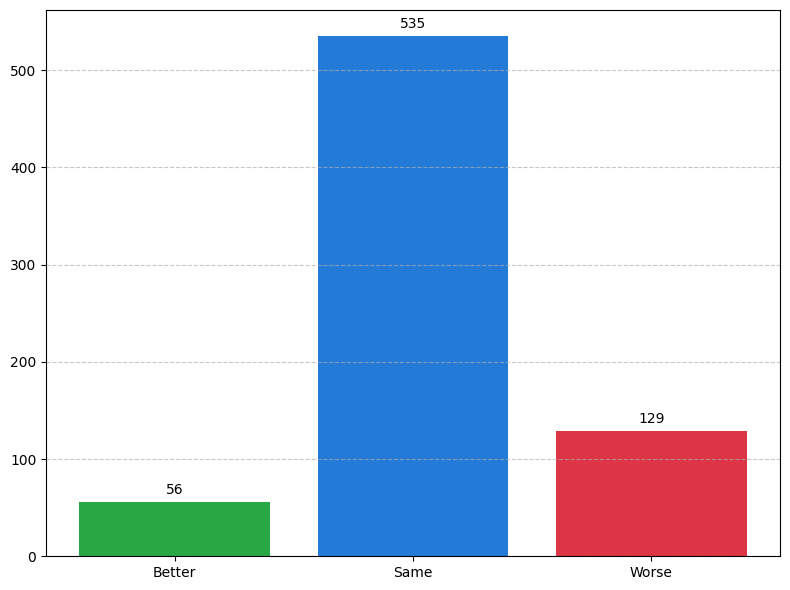
\includegraphics[width=0.9\columnwidth]{tesi/output2} 
    \caption{Confronto GA con soluzione aziendale}
\end{figure}

Il confronto con la soluzione aziendale è fatto prendendo la soluzione migliore ottenuta per ogni istanza dal genetico e la soluzione migliore ottenuta per ogni istanza dalla soluzione aziendale.

La Figura 6.1 mostra un grafico a barre in cui nell'asse y è presente il numero delle istanze, mentre, nell'asse x: 'Better' indica le istanze che hanno ottenuto un risultato migliore con GA, 'Same' indica le istanze che hanno ottenuto lo stesso risultato sia con GA che con la soluzione aziendale e 'Worse' indica le istanze che hanno ottenuto un risultato peggiore con GA.

Dalle due soluzioni viene confrontata la quantità di scarto totale prodotto:
\begin{itemize}
    \item 56 istanze eseguite con GA hanno ottenuto una soluzione che ha prodotto meno scarto rispetto dalla soluzione aziendale;
    \item 535 istanze hanno ottenuro lo stesso risultato;
    \item 129 istanze hanno ottenuto un risultato peggiore rispetto alla soluzione aziendale.
\end{itemize}

Quindi complessivamente la soluzione aziendale produce un maggior numero di soluzioni migliori per le istanze usate per il confronto.

\subsection{Altri test} \hypertarget{chiara3}{}

È stato tentato anche un aumento del \emph{pilot\_method\_prob} a 0,5 (50\%) ma ha prodotto risultati peggiori, infatti l'aumento del costo computazionale per l'esecuzione di ogni generazione, rispettando il criterio di arresto a 30 secondi, non ha permesso per alcune istanze di generare abbastanza generazioni per trovare soluzioni migliri che invece, con \emph{pilot\_method\_prob} uguale a 0,1 erano state trovate.

Nella generazione della popolazione iniziale sono stati provati anche altri criteri di ordinamento oltre ad \emph{AREA\_DESCENDING}, come: \emph{LONGER\_SIDE\_DESCENDING} (dal lato lungo maggiore a quello minore), \emph{PERIMETER\_DESCENDING} (dal perimetro maggiore al miniore) e \emph{SIDE\_DIFF\_DESCENDING} (dall'\emph{item} con meno differenza fra altezza e lunghezza a quello con più differenza). Questi criteri di ordinamento hanno ottenuto risultati peggiori (anche utilizzati in combinazione fra di loro e con \emph{AREA\_DESCENDING}) quindi sono stati scartati [\hyperlink{bibliografia}{9}]. 